\label{sec:Res}
\section*{Results}

Explain pattern of variability, underlines importance of species effect for growth and trait \missfig

However, species effect can't explain everything, tested for spatial auto-correlation.

Then, compared different growth models.

Examined link of predicted AGR with such model and distance to species average.

\begin{figure}[h!]
	\centering
	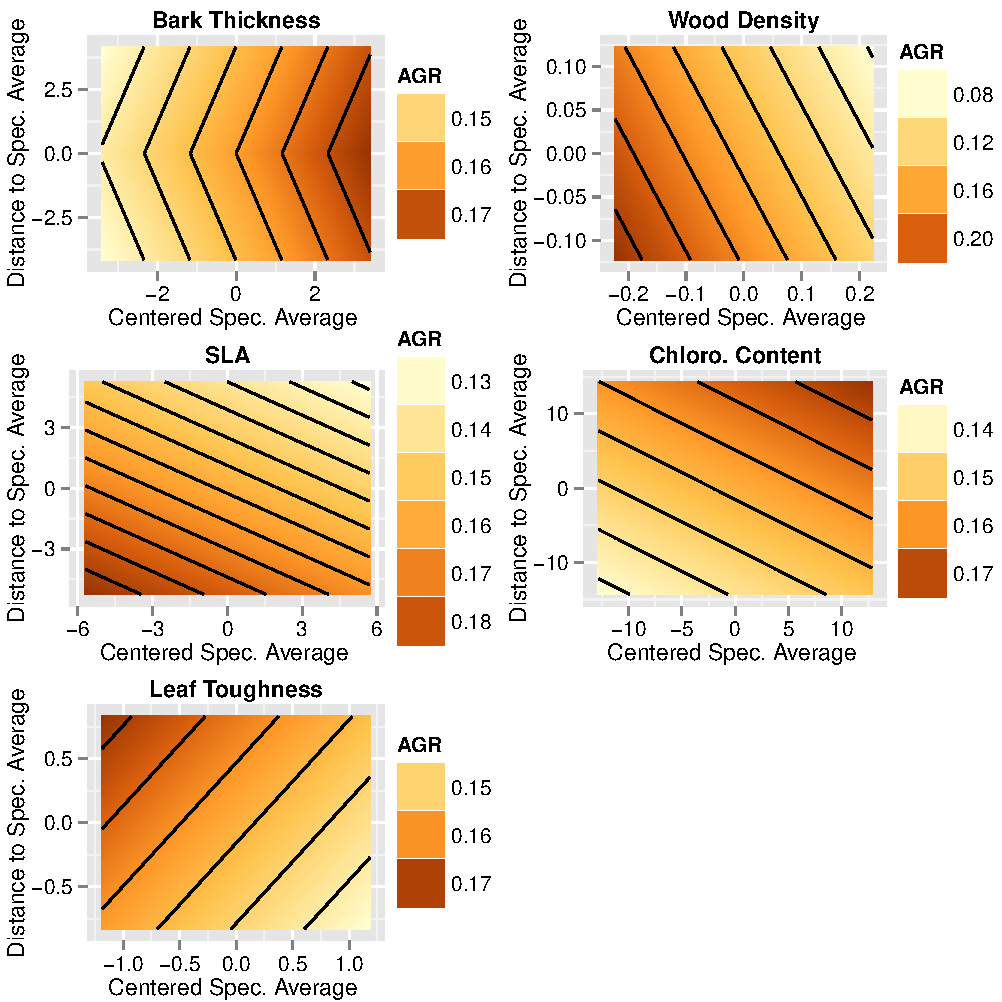
\includegraphics{figures/Sel_Traits_Simul_Pred_AGR_2015-05-22.pdf}
	\caption{\textbf{Simulations of species trait and predictions of AGR with growth models.} Surface plots of predicted AGR of simulated range of data: X-axis, centered species average trait (species average trait minus mean of all species average trait); Y-axis, individual distance to species average trait. Black lines are equal-AGR lines over the surface. For traits detail see~\autoref{tab:seltraits}.}
	\label{fig:simul}
\end{figure}